\chapter{Arkitektur}

% Beskrivelse af den overordnede systemarkitektur. Her skal SysML blok diagrammer benyttes. Der gives et overblik over systemets arkitektur med udgangspunkt og reference til jeres systemarkitektur dokument.

I dette afsnit beskrives den overordnede arkitektur for systemet. Systemets arkitektur har dannet ramme for design og senere implementering. Til at beskrive systemets arkitektur bruges 4+1 modellen som kan ses på figur~\ref{fig:41model}. Modellen er udviklet af Philippe Kruchten~\cite{fcgss2007}. Modellen indeholder fire views samt et user-story eller use-cases view.

\begin{itemize}
	\item \textbf{Logical view} - End-user funktionalitet
	\begin{itemize}
		\item Klassediagrammer, Package diagram, State machine diagram.
	\end{itemize}
	\item \textbf{Process view} - Adfærd og performance
	\begin{itemize}
		\item Activity diagram, Sekvens diagram.
	\end{itemize}
	\item \textbf{Implementation/Development view} - Udviklerperspektivet
	\begin{itemize}
		\item Component diagram.
	\end{itemize}
	\item \textbf{Physical view} - Fysiske bindinger i systemet
	\begin{itemize}
		\item Deployment diagram.
	\end{itemize}
\end{itemize}

\begin{figure}[h]
	\centering
	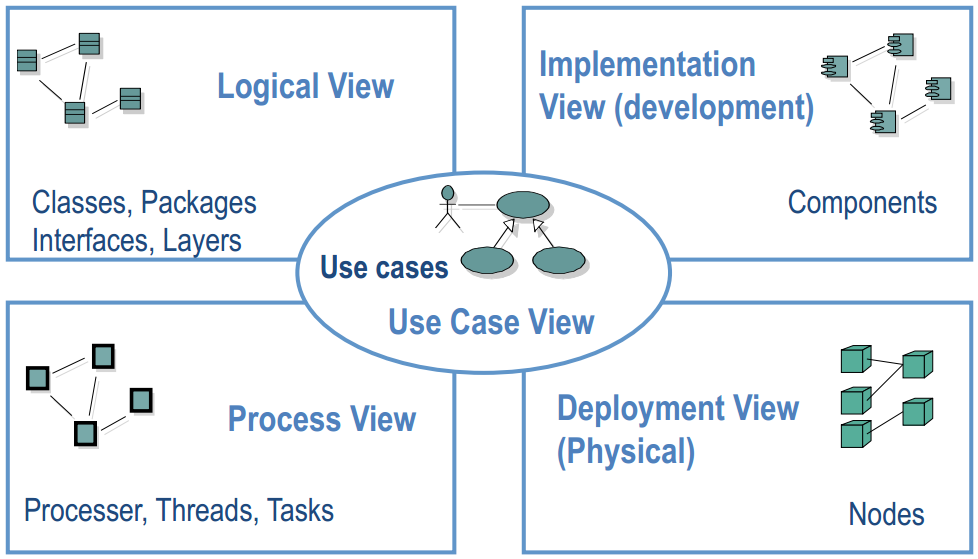
\includegraphics[width=0.9\linewidth]{figs/arkitektur/41model}
	\caption{$4+1$ Arkitektur modellen \cite{flylib}}
	\label{fig:41model}
\end{figure}

\section{Logical view}
\todo{Skriv kort om viewet.}
I 4+1 arkitekturen kan det logiske view repræsenteres med et pakkediagram.
På figur~\ref{fig:packageDiagram} ses projektets pakkediagram. På dette diagram vises de forskellige pakker i systemet, dog uden de klasser som de indeholder. Se dokumentationen for fuldt pakkediagram\todo{indsæt reference til dokumentation}.
Pakkediagrammet har til formål at vise systemets afhængigheder. Disse er vist med en stiplet pil. En fuldoptrukket linje med + betyder "\textit{nested} og altså at pakken er indeholdt i den anden pakke. Pakken \textit{External DLL's} er eksterne afhængigheder, såsom library filer og DLL'er der bruges.

\begin{landscape}
	\begin{figure}[H]
		\centering
		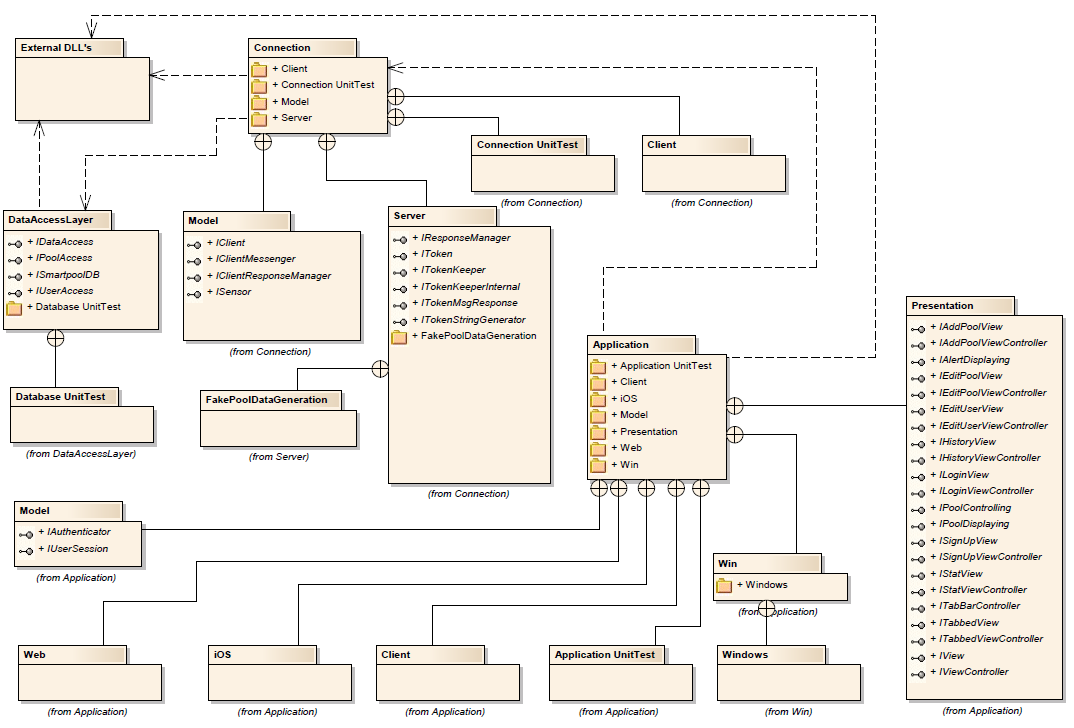
\includegraphics[width=\linewidth]{figs/arkitektur/packageDiagramNoImpl.PNG}
		\caption{Package model - Implementation/Development view}
		\label{fig:packageDiagram}
	\end{figure}
\end{landscape}

\section{Process view}
Dette view beskriver brugerens typiske anvendelse af programmet. Hvilke beslutninger brugeren stilles overfor, samt de forskellige valg og situationer. Dette er beskrevet via et activity diagram vist på figur~\ref{fig:ActivityDiagram}

\begin{figure}
\centering
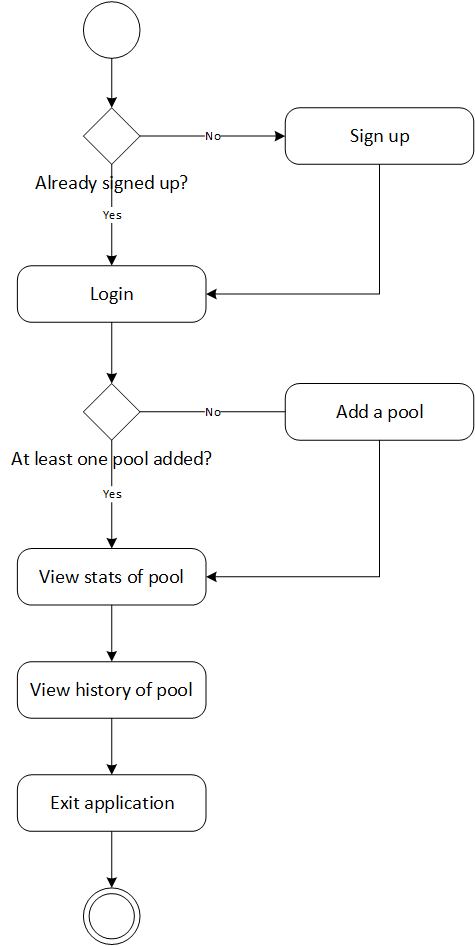
\includegraphics[width=0.55\linewidth]{figs/arkitektur/ActivityDiagram.PNG}
\caption{Activity diagram}
\label{fig:ActivityDiagram}
\end{figure}


\section{Implementation/Development view}
\todo{Skriv kort om development viewet.}

\begin{figure}
\centering
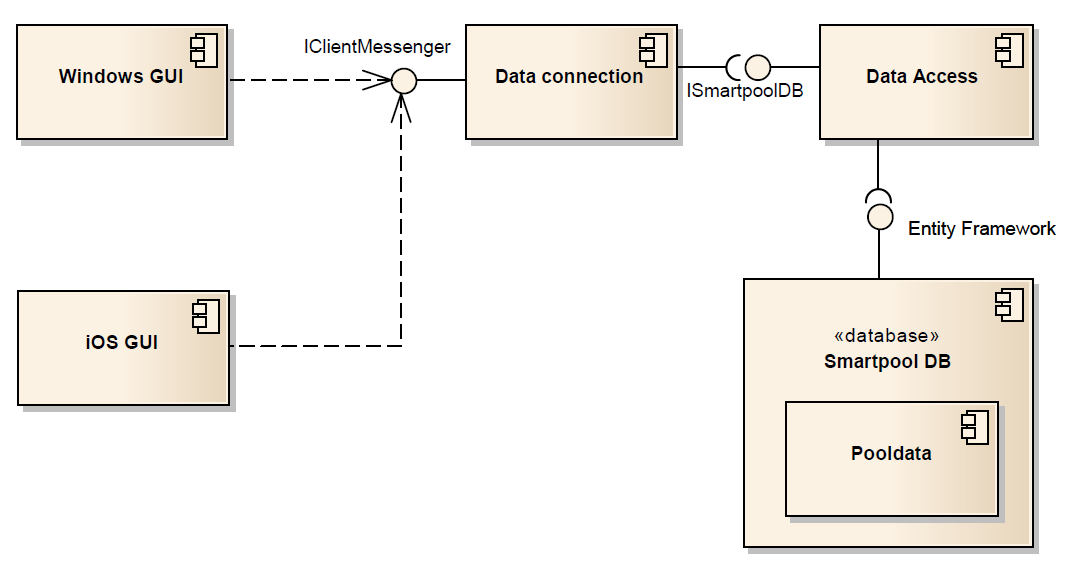
\includegraphics[width=0.7\linewidth]{figs/arkitektur/componentModel}
\caption{Component model for Smartpool systemet}
\label{fig:componentModel}
\end{figure}

Med component diagrammet på figur~\ref{fig:componentModel} er det forsøgt at vise de forskellige software komponenter, og de porte eksponeres. Windows og iOS GUI'erne bruger begge database forbindelsen, som bruger Data Access lagets interface ISmartpoolDB. Data access laget kommunikerer med den egentlige database vha. Entity Frameworket.

\section{Physical view}
\todo{Skriv kort om development viewet.}
 
Deployment diagrammet har til formål at vise systemets hardware (Klienter, servere og databaser), og hvordan de kommunikerer. Da Smartpool systemet er udviklet til flere typer af kienter, herunder iOS, Windows og Internet browsere giver deployment diagrammet god indsigt i hvordan elementerne hænger sammen.
På figur \ref{fig:deploymentView} ses projektets deployment diagram.

\begin{figure}
	\centering
	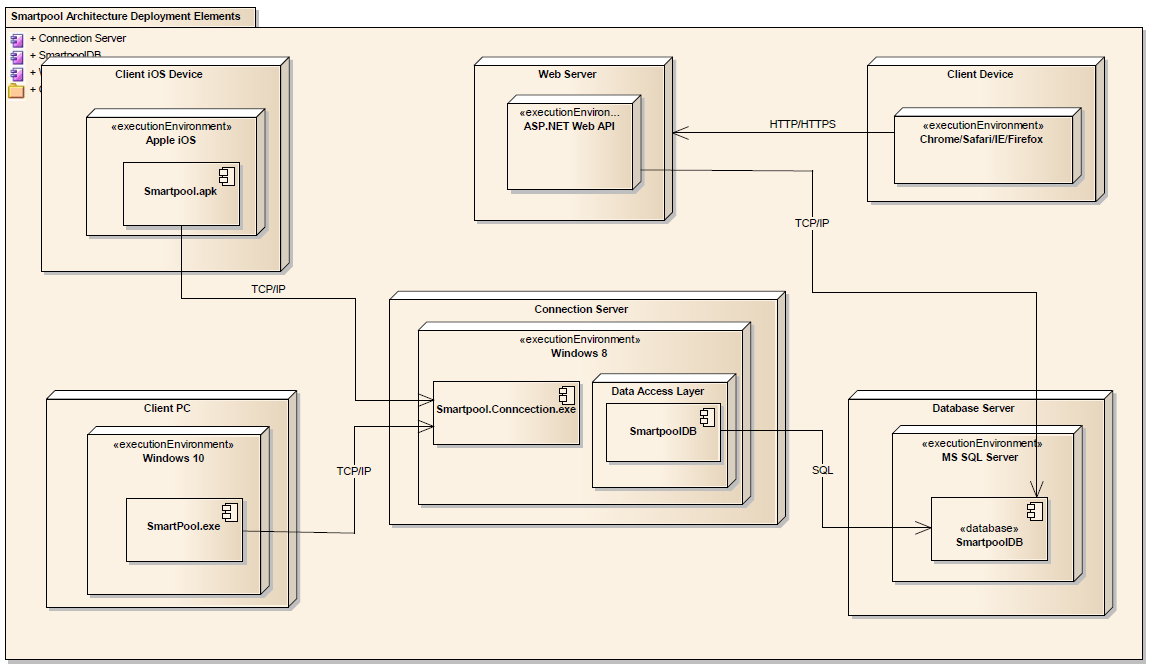
\includegraphics[width=\linewidth]{figs/arkitektur/deploymentView.PNG}
	\caption{Deployment diagram - Physical view}
	\label{fig:deploymentView}
\end{figure}

\section{Use case/User story view}
Til dette prokjekt er der brugt user stories til at beskrive systemets brugsscenarier. Disse User Stories kan ses på \todo{reference til US} hvor de er opstillet i en tabel.

